% Template for ICIP-2013 paper; to be used with:
%          spconf.sty  - ICASSP/ICIP LaTeX style file, and
%          IEEEbib.bst - IEEE bibliography style file.
% --------------------------------------------------------------------------
\documentclass{article}
\usepackage{spconf,amsmath,graphicx}
\usepackage{url}
\usepackage[spanish]{babel}
\selectlanguage{spanish}
\usepackage[utf8]{inputenc}

% Example definitions.
% --------------------
\def\x{{\mathbf x}}
\def\L{{\cal L}}

% Title.
% ------
\title{Video surveillance for road traffic monitoring}
%
% Single address.
% ---------------
\name{Adrià Ciurana, Guim Perarnau and Pau Riba} % \thanks{Thanks to XYZ agency for funding.}}
\address{Universitat Politècnica de Catalunya\\ Master in Computer Vision, Computer Science}
%
% For example:
% ------------
%\address{School\\
%	Department\\
%	Address}
%
% Two addresses (uncomment and modify for two-address case).
% ----------------------------------------------------------
%\twoauthors
%  {A. Author-one, B. Author-two\sthanks{Thanks to XYZ agency for funding.}}
%	{School A-B\\
%	Department A-B\\
%	Address A-B}
%  {C. Author-three, D. Author-four\sthanks{The fourth author performed the work
%	while at ...}}
%	{School C-D\\
%	Department C-D\\
%	Address C-D}
%
\begin{document}
%\ninept
%
\maketitle
%
\begin{abstract}
This article presents an algorithm for video surveillance devoted to road traffic monitoring. The proposed approach starts from the raw video of the road and ends with an estimation of the velocity for each car appearing in the images. Here, we present a detailed analysis for every step of the proposed solution and an evaluation for the whole pipeline. Moreover, we will face different problems such as camera jittering or dynamic background.
\end{abstract}

\begin{keywords}
Video Analysis, Video Surveillance, Background Estimation, Optical Flow, Kalman Filter
\end{keywords}
%
\section{Introduction and Motivation}
\label{sec:intro}

Nowadays, video surveillance is a hot topic in the field of computer vision. Using this kind of techniques allows not only to get lots of visual data but to analyze them automatically. In this work we have faced the problem of road traffic monitoring. Lots of other applications have been proposed for video surveillance in other scenarios (such as \cite{lipton2002}), but as Computer Vision Master students, we wanted to apply all the theoretical knowledge acquired during this course to make our own system. In our case we have chosen a straightforward approach that is based on strong assumptions and constraints (explained in Section \ref{sec:method}) so as to simplify the implementation of the video surveillance.

The rest of this paper is organized as follows. First, Section \ref{sec:method} describes all the steps done for creating our system. In Section \ref{sec:eval} we show the obtained results. Finally Section \ref{sec:conclusions} draws the conclusions and future work.

\section{Methodology}
\label{sec:method}

The proposed approach is constructed using different modules that we will explain in detail. Firstly, the foreground that contains the objects that we want to monitor must be segmented. Afterwards, we can detect the objects -- cars in our case -- and track them. From the tracking -- and given a real measure of the distance introduced by the user -- we can estimate the real velocity of the vehicles. The assumptions made for our applications are the following:
\begin{itemize}
	\item The user has to mark the lines of the road in order to calculate the homography based on the vanishing point. Also, the user has to indicate the relationship between a pixel and the real distance. That is, for example, how many pixels equals a meter (used in Subsection \ref{subsec:vel}).
    \item It is assumed that there won't be any occlusions in the sequences. If there are, our algorithm could track inaccurately.
\end{itemize}

\subsection{Background estimation}
\label{subsec:back}

Estimating the background is of key importance to the proposed technique. Three main approaches have been tested: two statistical models based on one Gaussian per pixel (Subsection \ref{subsec:sgGaus}) and a third based on a mixture of Gaussians (Subsection \ref{subsec:st_gr}). Then, color information has been added to improve the previous estimation. Thus, until Section \ref{subsec:color} we will be talking about gray-scale images.

\subsubsection{Single Gaussian per pixel}
\label{subsec:sgGaus}

The previously mentioned statistical models share the same idea, which consists of one Gaussian function to model each background pixel. From the first frames of our sequences we can estimate the Gaussian parameters \(\mu\) and \(\sigma\) for each pixel. For every frame, we define a pixel \(I_i\) as foreground if the following condition is fulfilled:

\begin{equation}
|I_i-\mu_i| \geq \alpha(\sigma_i+2) \mbox{ for all} \operatorname{pixel} i
\end{equation}

At this point, this model can be divided between a non adaptive or adaptive approach.

\begin{itemize}
	\item \emph{Non Adaptive}: \(\mu\) and \(\sigma\) are static -- they do not adapt. They are calculated only once during a training process. This approach has some drawbacks.
	\item \emph{Adaptive or recursive}: the Gaussians are adapted using the segmented background in the previous frame. Therefore, we will adapt to slow changes in the background, such as illumination. This technique uses a parameter \(\rho\) to control the adaptation speed. Then, the adaption is performed\(\mbox{ for all} \operatorname{pixel} i \in \operatorname{Background}\) following the equations below:
    \begin{equation}
      \begin{aligned}
            \mu_i &= \rho I_i+ (1-\rho)\mu_i\\
            \sigma_i &= \rho(I_i-\mu_i)^2+(1-\rho)\sigma_i^2
      \end{aligned}
    \end{equation}
\end{itemize}

\subsubsection{Stauffer and Grimson}
\label{subsec:st_gr}
Stauffer and Grimson \cite{stauffer1999} have proposed a technique for background estimation that uses a Gaussian Mixture Model (GMM) to model foreground objects. As the single Gaussian method, S\&G is based on the temporal observation of the pixels. 
Each pixel is assigned to its nearest Gaussian. If the Gaussian models foreground (background), the pixel will be detected as foreground (background). It is necessary to manually set the number of Gaussians used (normally between 3 and 6) to adapt to data. 
The authors claim that this technique reliably deals with lighting changes, repetitive motions from clutter, and long-term scene changes (for ex. if a car parks and remains still will eventually detected as background).

\subsubsection{Color space}
\label{subsec:color}

Originally, we only used gray-scale images. However, the original input images are in color, meaning that if we convert them to gray-scale, we are losing information that we could benefit from. Thus, we have tested three different color spaces: RGB, YUV and CIE-Lab \cite{hunter1948}. The first one is the most common color space but it has some drawbacks that other spaces try to correct. For instance, YUV space is focused on taking human perception into account whereas CIE-Lab aims to separate luminescence from the chromatic channels.

\subsection{Foreground segmentation}
\label{subsec:fore}

Once the background has been estimated, we want to avoid the parts that are miss-classified as foreground due to noise (camera jittering produced by the wind) or dynamic background (rustling leaves). The correction proposed in this Section differs from Section \ref{subsec:back} because it uses neighbor pixels information, whereas the background estimation uses locally per-pixel information in the time domain. We propose to apply mathematical morphology to correctly eliminate miss-classifications using three operations:

\begin{enumerate}
	\item \emph{Area filtering}: in order to delete noise from the background produced by camera movements, wind, etc. However, it could mistakenly delete foreground blobs.
    \item \emph{Closing}: in order to join blobs of the same object that could be separated.
    \item \emph{Hole filling}: fill holes of foreground objects in the segmentation.
\end{enumerate}

Figure \ref{fig:res} shows the pipeline for a frame from the input image to the foreground segmentation. Figure \ref{fig:res}(a) represents one frame of a video sequence from which \(\mu\) and \(\sigma\) for background estimation are known. Thus, the background can be estimated giving the mask showed in Figure \ref{fig:res}(b). Afterwards, the mask is refined performing a foreground estimation by means of morphological filtering (Figure \ref{fig:res}(c).

% Below is an example of how to insert images. Delete the ``\vspace'' line,
% uncomment the preceding line ``\centerline...'' and replace ``imageX.ps''
% with a suitable PostScript file name.
% -------------------------------------------------------------------------
\begin{figure}[htb]

\begin{minipage}[b]{1.0\linewidth}
  \centering
  \centerline{\includegraphics[width=0.75\textwidth]{fig/in001234}}
%  \vspace{2.0cm}
  \centerline{(a) Input image 'in001234.jpg' from 'Highway' sequence}\medskip
\end{minipage}
%
\begin{minipage}[b]{.48\linewidth}
  \centering
  \centerline{\includegraphics[width=\textwidth]{fig/block1}}
%  \vspace{1.5cm}
  \centerline{(b) Background estimation}\medskip
\end{minipage}
\hfill
\begin{minipage}[b]{0.48\linewidth}
  \centering
  \centerline{\includegraphics[width=\textwidth]{fig/block2}}
%  \vspace{1.5cm}
  \centerline{(c) Foreground segmentation}\medskip
\end{minipage}
%
\caption{Example of the background estimation (section \ref{subsec:back}) and foreground segmentation (Section \ref{subsec:fore}) for an input image of the 'Highway' sequence (database info. in Section \ref{subsec:database}).}
\label{fig:res}
%
\end{figure}

\subsection{Stabilization}

An estimation of the optical flow of the sequence using either block matching or Lucas-Kanade \cite{lucas1981iterative} can be applied in order to perform an image stabilization so as to avoid the miss-segmentation and noise produced by camera jittering. For the block matching algorithm, the block division size is the most relevant parameter. There can happen that pixels that are moving in different directions fall in the same block, making the estimated flow to be inaccurate. On the other hand, L-K does not divide the image by blocks but allows each pixel to have its own direction using the Taylor approximation.
However, the performance of the background segmentation falls and it has been discarded.

\subsection{Tracking}

For tracking purposes, two main approaches have been tested. First an algorithm based on Kalman filter \cite{kalman1960new} is used. This algorithm is optimal for linear dynamical models under the assumption of Gaussian noise. Then another technique based on a stack denoising autoencoder for representing features and neural networks for classification \cite{wang2013nips} has also been tested.

Both techniques have been implemented as the tracking of a bigger system of lives. There, each blob that is tracked by one of these algorithms have their own life-cycle. For instance, a blob that do not move will be classified as inactive and will lose lives for each new frame. Afterwards, if this object loses all his lives, it is deleted. Therefore, the proposed system avoids the background noise or miss classified blobs due to a camera movement in one frame.

\begin{figure}[!htb]
	\centering
	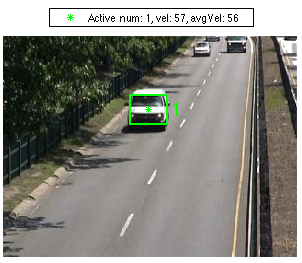
\includegraphics[width=0.4\textwidth]{fig/traker_car}
    \caption{Car tracked in a frame from the 'Highway' sequence.}
    \label{f:trackcar}
\end{figure}

\subsection{Velocity estimation} 
\label{subsec:vel}

Firstly, let us remark that in a non orthogonal point of view images the objects will move in different velocities depending on their distance from the camera, no matter if their real velocity is constant. To solve that problem, an homography matrix can be defined. The proposed approach asks the user for two lines that are parallel in the real world and computes their vanishing point. Once the homography is computed, the image can be projected in a bird's-eye perspective, where the estimation of the speed will not be dependent on the car position. Taking the trackers from the previous section, we can easily estimate the velocity of the moving object in pixels per frame through the proposed homography \(\operatorname{norm}(\vec{cd})\). Then, taking a fix reference from the real world \(\vec{ab}\) and knowing their length (\(\operatorname{dist}(a,b)\) given by the user) the scale factor is computed:

\begin{equation}
\operatorname{dist}(c,d)=\operatorname{norm}(\vec{cd})\frac{\operatorname{dist}(a,b)}{\operatorname{norm}(\vec{ab})}
\end{equation}

In road sequences, we can use an approximation of the length of the road central lines. This length can be easily obtained from \cite{USfedguide}. Hence, it is defined that the mentioned lines measure 10 feet or 3.04 meters. Using this information and a scale factor \(\alpha\) the real speed in kilometers per hour is estimated. Figure \ref{fig:homo} shows an example for the homography.

\begin{figure}[htb]
\begin{minipage}[b]{.48\linewidth}
  \centering
  \centerline{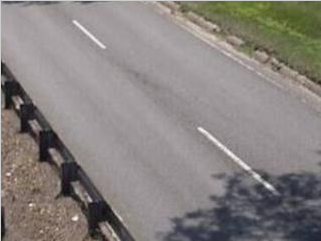
\includegraphics[width=\textwidth]{fig/Traffic}}
%  \vspace{1.5cm}
  \medskip
\end{minipage}
\hfill
\begin{minipage}[b]{0.48\linewidth}
  \centering
  \centerline{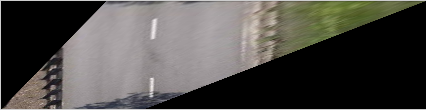
\includegraphics[width=\textwidth]{fig/Traffic_h}}
%  \vspace{1.5cm}
\medskip
\end{minipage}
%
\caption{Example of the homography transformation for the Traffic sequence.}
\label{fig:homo}
%
\end{figure}

Figure \ref{f:trackcar} shows an example of the proposed tracker with the computed velocity. The system keeps track of the velocity in each point and their average. The velocity estimated can produce bigger jumps due to segmentation problems or other cars or shadows. Hence, we also compute and show the average speed.

\section{Evaluation} \label{sec:eval}
\subsection{Database}
\label{subsec:database}

For evaluation purposes, we used the Change Detection Benchmark Dataset \cite{wang2014cdnet} which is an open database for foreground segmentation purpose. From this dataset, three sequences have been used. Table \ref{t:dataset} shows the frames that have been used for different types of evaluation.

\begin{table}
  \begin{center}
  	\caption{Set of frames for evaluation purposes.}
    \label{t:dataset}
    \begin{tabular}{c | c | c}
      \textbf{Sequence} & \textbf{Frame Range} & \textbf{Type}\\
      \hline
      \emph{Highway} & 1050 - 1350 & Baseline\\
      %\emph{Fall} & 1460 - 1560 & Dynamic background\\
      \emph{Traffic} & 950 - 1050 & Camera jitter\\
    \end{tabular}
  \end{center}
\end{table}

%\subsection{Metrics}

%The results will be presented in terms of F1-score, precision-recall curve and area under the curve (AUC). This metrics are computed pixel-wise using the ground truth masks.

%\begin{equation}
%\operatorname{F1-score} = 
%\frac{2\operatorname{Precision} \cdot \operatorname{Recall}}%{\operatorname{Precision} + \operatorname{Recall}}
%\end{equation}

\subsection{Results}

In this Section we will present the results for all the modules. Moreover, the final estimation of the speed is also presented for different sequences\footnote{\url{https://youtu.be/5w7WQJvfClA}}.

\subsubsection{Background Estimation}

As it has been explained in subsection \ref{subsec:back}, the idea is to distinguish between background and foreground. Figure \ref{f:compback} shows a comparison in terms of F1-Score for three sequences setting the parameters \(\alpha\) and \(\rho\). It is clear, that the best technique (in average) for our case of study is the adaptive single Gaussian per pixel.

\begin{figure}[!htb]
	\centering
	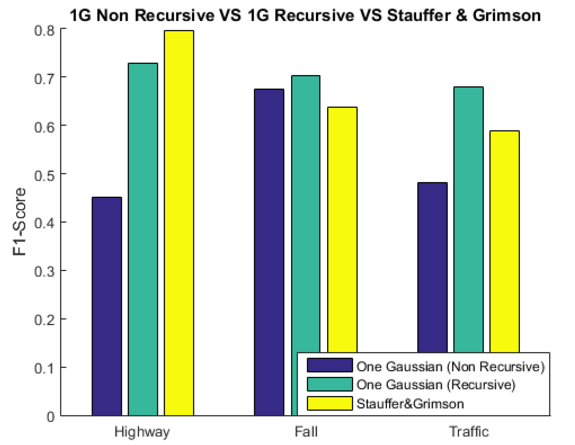
\includegraphics[width=0.4\textwidth]{fig/task1_comparisonMethods}
    \caption{Comparison of background segmentation techniques for three sequences.}
    \label{f:compback}
\end{figure}

Hence, this work has been devoted to improve this segmentation using color and foreground segmentation. Table \ref{t:bckauc} shows a global measure (AUC) depending of \(\alpha\) and setting \(\rho\) to the best value obtained for each sequence (0.2 for Highway and Traffic and 0.1 for Fall sequence). Using a global measure gives us more information about the stability of the proposed technique.

For the foreground segmentation, also shown in Table \ref{t:bckauc}, we found that the best parameters are \(\operatorname{connectivity}=4\) for the hole filling, \(\operatorname{p}=5\) for the closing and \(\operatorname{area}=300\) for the area filtering. Shadow removal algorithm has also been tested but have been shown to decrease the performance of the system deleting foreground instead of background. Figure \ref{f:shadow} shows the shadow issues where it is segmented as foreground. Moreover, for the background colors and shadows, it is split into two blobs and both are classified as a car. 

\begin{figure}[!htb]
	\centering
	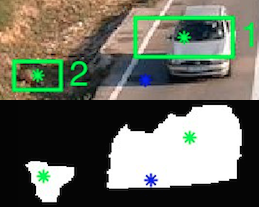
\includegraphics[width=0.2\textwidth]{fig/shadowProblem}
    \caption{Shadows are still an issue for the proposed approach.}
    \label{f:shadow}
\end{figure}

\begin{table}
\caption{Area under the precision-recall curve for three sequences and their average. Column 2 corresponds to the AUC for the background estimation and the last one indicates the AUC for the foreground estimation and the improvement with respect the previous column.}
\begin{center}
\begin{tabular}{c | c c}
& \textbf{Back. Est.} & \textbf{Fore. Seg.}\\
\hline
\emph{Highway} & 0.7539 & 0.8423 (+11\%)\\
\emph{Fall} & 0.7954 & 0.9526 (+19\%)\\
\emph{Traffic} & 0.7081 & 0.7807 (+10\%)\\
\textbf{Average} & 0.7525 & 0.8585 (+14\%)\\
\end{tabular}
\end{center}
\label{t:bckauc}
\end{table}

\subsubsection{Road Traffic Monitoring}

The final objective of this work is to monitor, track and count the vehicles in some roads. Hence, we have to identify each car and be able to get an estimation of the speed along the road stretch.

Table \ref{t:speedest} shows some examples of detected vehicles for each sequence and their corresponding speed. For the Highway sequence 29 cars have been detected (26) whereas for the Traffic sequence 23 cars have been detected (30).

The speed provided in Table \ref{t:speedest} is the average of all instant speeds where the car is detected. In order to test the accuracy of the velocity estimation, a new sequence have been recorded with one of the cars moving at constant speed (40km/h or 50km/h depending on the sequence).

\begin{table}
\caption{Relations between vehicles and their speed (km/h) in two sequences}
\begin{center}
\begin{tabular}{c c}
Sequence & \textbf{Highway} \\
\hline
& \textbf{Est. speed}\\
Car 1 & 62.0090\\
Car 2 & 88.1962\\
Car 3 & 54.2807\\
Car 4 & 53.8650\\
\end{tabular}
\quad
\begin{tabular}{c c}
Sequence & \textbf{Traffic}\\
\hline
& \textbf{Est. speed}\\
Car 1 & 69.5027\\
Car 2 & 68.4294\\
Car 3 & 57.3601\\
Car 4 & 61.688\\
\end{tabular}
\end{center}
\label{t:speedest}
\end{table}



\section{Conclusions and future work}
\label{sec:conclusions}

During this work, a video surveillance framework has been presented. Each module has been discussed separately and its performance evaluated. Finally, the whole system has been presented to be able to count and track the cars and estimate their velocity.

The work proposed has shown to get good results under strict assumptions. Future work should be focused on improve the techniques for video stabilization and shadow removal. Moreover, another key point to increase the performance of the proposed pipeline could be a module to segment objects in the foreground mask in order to avoid problems related with occlusions. Furthermore, other state of the art stabilization and shadow removal techniques could give an important increase of the performance \cite{kopf2014first}.

% To start a new column (but not a new page) and help balance the last-page
% column length use \vfill\pagebreak.
% -------------------------------------------------------------------------
%\vfill
%\pagebreak

% References should be produced using the bibtex program from suitable
% BiBTeX files (here: strings, refs, manuals). The IEEEbib.bst bibliography
% style file from IEEE produces unsorted bibliography list.
% -------------------------------------------------------------------------
\bibliographystyle{IEEEbib}
\bibliography{references/strings,references/refs}

\end{document}
